\chapter{Introduccion} \chapterlabel{Informe/1-Introduccion} \label{cap:Introducción}


\noindent \colorbox{yellow}{Ver de poner una intro general de levitación magnetica y la importancia de los sistemas de control}

\noindent El desarrollo de este sistema de levitación magnética surge como idea de la cátedra Sistemas de Control de la carrera de Ingeniería Electrónica, con el objetivo de disponer de una planta de control para realizar prácticas en clase. Una primera versión de este dispositivo fue desarrollada y construída por la cátedra. Los integrantes de este proyecto tuvieron la oportunidad de realizarle pruebas y modificaciones durante el cursado de la asignatura. Sin embargo, no se pudo lograr que el dispositivo funcionara correctamente al finalizar la cursada. Por este motivo, se propuso hacer un rediseño de todas las etapas que componen al sistema en el marco de un proyecto final.



\section{Alcance del proyecto}

\noindent El objetivo de este proyecto es diseñar un sistema de levitación magnética a partir de un electroimán de laminación normalizada con núcleo tipo “E''. Este sistema integra las etapas de driver de corriente de potencia, estimación de distancia de levitación, y control de la planta. Estas dos últimas deben implementarse tanto en forma analógica como digital.

\noindent Este documento contempla el proceso de diseño y modelado de todas las etapas pertenecientes al sistema, junto con su implementación circuital y simulaciones. Además, se realiza el diseño del circuito impreso de la placa de control.



\section{Contexto del proyecto}

\noindent El proyecto comenzó en junio del 2020. Inicialmente tenía como objetivo el diseño y la construcción de un prototipo funcional que permitiera a los alumnos de la asignatura de Sistemas de Control realizar mediciones y observar el comportamiento de las distintas etapas que componen el sistema. Sin embargo, debido a los retrasos ocasionados por la pandemia (COVID-19), los costos asociados a la fabricación de la placa de control y sus componentes, sumado a la  necesidad de no extender indefinidamente el proyecto, se optó por acotar el alcance sólo al diseño teórico de todas las etapas y del circuito impreso.

\noindent Se espera que en el futuro se pueda construir el sistema de levitación magnética para que sirva como herramienta para los alumnos, de forma tal que les permita experimentar y afianzar los conceptos teóricos adquiridos durante el transcurso de la cursada.



\section{Descripción del dispositivo}

\noindent El producto está compuesto por dos partes principales: un electroimán y una placa de control. El electroimán tiene dos piezas formadas por láminas de acero apiladas: una con forma de “E”, que tiene un cable bobinado en su rama central y otra con forma de “I” que es atraída por la primera mediante una fuerza electromagnética. Esta fuerza es regulada por la placa de control, que mantiene la distancia de separación ($Y_{g}$) o “gap” de aire deseado entre ellas mientras el objeto que se desea hacer levitar se sujeta de la pieza en forma de “I”. Dicha separación puede ser modificada por el usuario entre $3\:mm$ y $5\:mm$ y el peso del objeto debe ser menor a $30\:Kg$. El sistema completo se muestra en la figura \ref{fig:img_Esquema-del-producto}.

\begin{figure}[H]
	\centering
	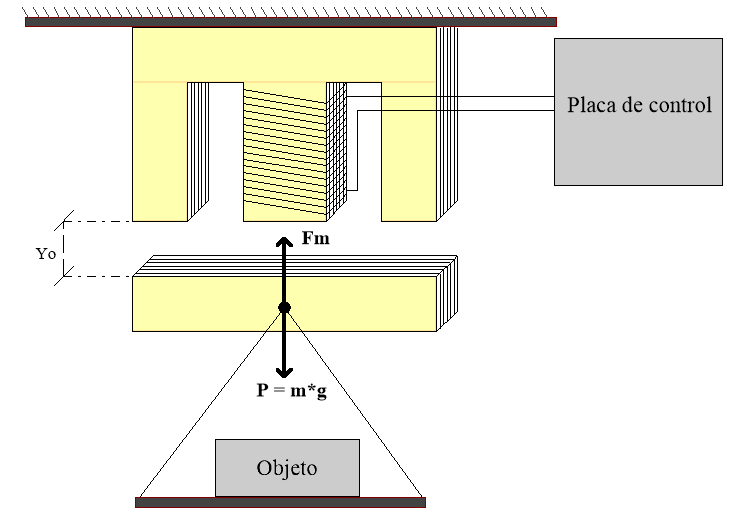
\includegraphics[width=\textwidth]{esquema-del-producto.png}
	\caption{Esquema del producto.}
	\label{fig:img_Esquema-del-producto}
\end{figure}

\noindent La fuerza electromagnética es regulada por la placa de control con el objetivo de mantener fija la distancia $Y_{g}$, a pesar de las perturbaciones que el sistema pueda recibir. 


\noindent El sistema solo ejerce control de posición en el eje vertical, por lo tanto no puede responder ante perturbaciones horizontales sobre el objeto.


\noindent El sistema está conformado por los bloques que se muestran en la figura \ref{fig:img_diagrama-en-bloques-del-sistema}. Se utilizan dos controladores distintos: uno analógico y otro digital. Cada uno de ellos se compone de un compensador y un estimador de posición.  El usuario decide cual de estas implementaciones ejerce el control mediante la utilización de un switch, por lo que solo una estará activa al mismo tiempo. El sistema analógico está formado por un conjunto de componentes pasivos y amplificadores operacionales, mientras que el digital está basado en un microcontrolador re-programable.

\begin{figure}[H]
	\centering
	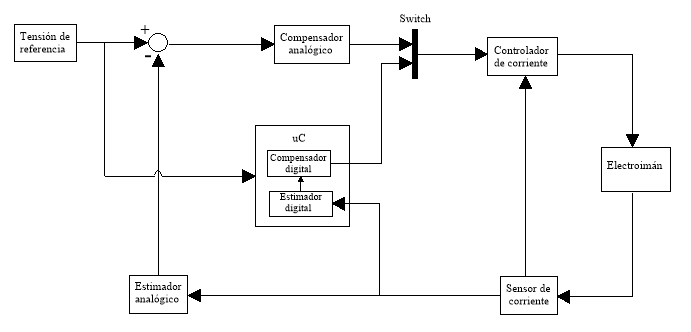
\includegraphics[width=\textwidth]{diagrama-en-bloques-del-sistema.png}
	\caption{Diagrama en bloques del sistema.}
	\label{fig:img_diagrama-en-bloques-del-sistema}
\end{figure}

\noindent El estimador de posición se encarga de entregar una tensión proporcional al gap de aire real a partir de la corriente que circula por el electroimán. El usuario puede modificar el gap de aire según desee mediante un potenciómetro presente en la placa de control. Tanto la implementación analógica como la digital reciben como entrada esta tensión. Luego, es comparada con la estimación y se utiliza como entrada para el compensador.

\noindent La función del compensador es garantizar la estabilidad del sistema. Esto lo logra al modificar la referencia del controlador de corriente mediante una acción de control. 

\noindent Por otro lado, el controlador de corriente se encarga de proveer corriente al electroimán de forma tal que le permita generar la fuerza electromagnética necesaria para mantener el gap de aire.
 